% Hlavicka pro protokoly z fyzikalniho praktika.
% Verze pro: LaTeX
% Verze hlavicky: 22. 2. 2007
% Autor: Ustav fyziky kondenzovanych latek
% Ke stazeni: www.physics.muni.cz/ufkl/Vyuka/
% Licence: volne k pouziti, nejlepe k vcasnemu odevzdani protokolu z Vaseho mereni.

\documentclass[a4paper,11pt]{article}

% Kodovani (cestiny) v dokumentu: utf-8
%\usepackage[cp1250]{inputenc}	% Omezena stredoevropska kodova stranka, pouze MSW.
\usepackage[utf8]{inputenc}	% Doporucujeme pouzivat UTF-8 (unicode).

%%% Nemente:
\usepackage[margin=2cm]{geometry}
\newtoks\jmenopraktika \newtoks\jmeno \newtoks\datum
\newtoks\obor \newtoks\skupina \newtoks\rocnik \newtoks\semestr
\newtoks\cisloulohy \newtoks\jmenoulohy
\newtoks\tlak \newtoks\teplota \newtoks\vlhkost
\usepackage{amsmath}
\usepackage{mathtools}
\usepackage{graphicx}
\usepackage{multirow}
\graphicspath{ {./images/} }
%%% Nemente - konec.


%%%%%%%%%%% Doplnte pozadovane polozky:

\jmenopraktika={Fyzikální praktikum 2}  % nahradte jmenem vaseho predmetu
\jmeno={Artem Gorodilov}            % nahradte jmenem mericiho
\datum={16. ~října  2023}        % nahradte datem mereni ulohy
\obor={Astrofyzika}                     % nahradte zkratkou vami studovaneho oboru
\skupina={Čt 8:00}            % nahradte dobou vyuky vasi seminarni skupiny
\rocnik={II}                  % nahradte rocnikem, ve kterem studujete
\semestr={I}                 % nahradte semestrem, ve kterem studujete

\cisloulohy={4}               % nahradte cislem merene ulohy
\jmenoulohy={Brownův pohyb a pohyblivost částic} % nahradte jmenem merene ulohy

\tlak={998}                   % nahradte tlakem pri mereni (v hPa)
\teplota={24.5}               % nahradte teplotou pri mereni (ve stupnich Celsia)
\vlhkost={38}               % nahradte vlhkosti vzduchu pri mereni (v %)

%%%%%%%%%%% Konec pozadovanych polozek.


%%%%%%%%%%% Uzitecne balicky:
\usepackage[czech]{babel}
\usepackage{graphicx}
\usepackage{amsmath}
\usepackage{xspace}
\usepackage{url}
\usepackage{indentfirst}
\usepackage{listings}
\usepackage{subcaption}
\usepackage{caption}
\usepackage{tabularx}
\usepackage[labelformat=parens,labelsep=quad,skip=3pt]{caption}

%%%%%% Zamezeni parchantu:
\widowpenalty 10000 \clubpenalty 10000 \displaywidowpenalty 10000
%%%%%% Parametry pro moznost vsazeni vetsiho poctu obrazku na stranku
\setcounter{topnumber}{3}	  % max. pocet floatu nahore (specifikace t)
\setcounter{bottomnumber}{3}	  % max. pocet floatu dole (specifikace b)
\setcounter{totalnumber}{6}	  % max. pocet floatu na strance celkem
\renewcommand\topfraction{0.9}	  % max podil stranky pro floaty nahore
\renewcommand\bottomfraction{0.9} % max podil stranky pro floaty dole
\renewcommand\textfraction{0.1}	  % min podil stranky, ktery musi obsahovat text
\intextsep=8mm \textfloatsep=8mm  %\intextsep pro ulozeni [h] floatu a \textfloatsep pro [b] or [t]

% Tecky za cisly sekci:
\renewcommand{\thesection}{\arabic{section}.}
\renewcommand{\thesubsection}{\thesection\arabic{subsection}.}
% Jednopismenna mezera mezi cislem a nazvem kapitoly:
\makeatletter \def\@seccntformat#1{\csname the#1\endcsname\hspace{1ex}} \makeatother

\begin{document}

\thispagestyle{empty}

{
\begin{center}
\sf 
{\Large Ústav fyzikální elektroniky PřF MU} \\
\bigskip
{\huge \bfseries FYZIKÁLNÍ PRAKTIKUM} \\
\bigskip
{\Large \the\jmenopraktika}
\end{center}

\bigskip

\sf
\noindent
\setlength{\arrayrulewidth}{1pt}
\begin{tabular*}{\textwidth}{@{\extracolsep{\fill}} l l}
\large {\bfseries Zpracoval:}  \the\jmeno & \large  {\bfseries Naměřeno:} \the\datum\\[2mm]
\large  {\bfseries Obor:} \the\obor  \hspace{40mm}  {\bfseries Skupina:} \the\skupina %
%{\bfseries Ročník:} \the\rocnik \hspace{5mm} {\bfseries Semestr:} \the\semestr  
&\large {\bfseries Testováno:}\\
\\
\hline
\end{tabular*}
}

\bigskip

{
\sf
\noindent \begin{tabular}{p{3cm} p{0.6\textwidth}}
\Large  Úloha č. {\bfseries \the\cisloulohy:} \par
\smallskip
$T=\the\teplota$~$^\circ$C \par
$p=\the\tlak$~hPa \par
$\varphi=\the\vlhkost$~\%
&\Large \bfseries \the\jmenoulohy  \\[2mm]
\end{tabular}
}

\vskip1cm

\section{Zadání}
    Provádět měření Brownova pohybu a ověřit platnost Einsteinova vztahu, kterým by se měla řídit částice ve stavebním bloku.
    \par Zaměřit na měření mobilitu volných elektronů v měděném vodiči navinutém kolem cylindrického jádra.
    \par
    \vspace{10px}
    \begin{minipage}[t]{0.5\textwidth} 
    \section{Teorie}
        \subsection{Brownův pohyb}
            V případě, že v kapalině existují mikroskopické částice, dochází k jejich pohybu způsobenému srážkami atomů kapaliny s těmito částicemi. Tento pohyb není zaznamenatelný, pokud jsou částice velké, neboť síly působící mezi atomy kapaliny se vyruší. Naopak, u malých částic tyto síly nejsou vykompenzovány, což vede k náhodnému pohybu, známému jako Brownův pohyb, a tento pohyb lze matematicky popsat Stokesovým zákonem. Jeho chování je také popsáno Einsteinovým zákonem: pokud sledujeme pozice částice v určených časových okamžicích, průměrný kvadratický posun částice je úměrný voleným časovým intervalům. K výpočtu tohoto jevu použijeme 2. Newtonův zákon, který dále upravíme pro naši specifickou situaci.
            \begin{equation}
                m \frac{d^2x}{dt^2} = F_1 + F_2
            \end{equation}
            kde $m$ je hmotnost částice, $F_1$ je celková síla a $F_2$ je odporová síla okolních molekul. 
            \par Pro sílu $F_2$ platí vztah:
            \begin{equation}
                F_2 = -k \frac{dx}{dt}
            \end{equation}
    \end{minipage}
    \hspace{10pt}
    \begin{minipage}[t]{0.5\textwidth} 
        Podle Stokesova zákona:
        \begin{equation}
            k = 6 \pi \eta r
        \end{equation}
        kde $\eta$ je viskozita kapaliny a $r$ je poloměr částice.
        \par Kombinací rovnic (1) a (2) a násobením na $x$ získáme: 
        \begin{equation}
            mx \frac{d^2x}{dt^2} = F_1x -kx \frac{dx}{dt}
        \end{equation}
        Dále vyjádříme první a druhý diferenciální člen
        \begin{equation}
           x \frac{d^2x}{dt^2} = \frac{1}{2} \frac{d^2}{dt^2} x^2 - \left(\frac{dx}{dt}\right)^2
        \end{equation}
        \begin{equation}
          x \frac{dx}{dt} = \frac{1}{2} \frac{dx^2}{dt}
        \end{equation}
        Zkombinujme všechny rovnice dohromady:
        \begin{equation}
          \frac{m}{2} \frac{d^2}{dt^2} x^2 - m\left(\frac{dx}{dt}\right)^2 = F_1 x - \frac{k}{2} \frac{dx^2}{dt}
        \end{equation}
        Jelikož nás pouze střední hodnoty zajímají, můžeme pro $F_1$, $x$ nastavit 0 a nadále si připomenout následující:
        \begin{equation}
            \frac{d}{dt}\left\langle x^2 \right\rangle = h
        \end{equation}
    \end{minipage}
    \newpage
    \begin{minipage}[t]{0.5\textwidth} 
        Pak:
        \begin{equation}
            \frac{m}{2} \frac{dh}{dt} - m \left\langle\frac{dx}{dt}\right\rangle
        \end{equation}
        Protože je druhý termín na pravé straně rovnice (9) dvojnásobkem průměrné kinetické energie částice. Použijeme-li teorii ideálního plynu na pohyb brownovské částice a zaměříme se pouze na jednu složku rychlosti ve směru osy 3, získáme následující vzorci:
        \begin{equation}
            \left\langle\frac{m\upsilon^2}{2}\right\rangle = \frac{3RT}{2N_A}
        \end{equation}
        \begin{equation}
           m \left\langle\frac{dx}{dt}\right\rangle = \frac{RT}{N_A}
        \end{equation}
        kde $N_A$ je Avogadrova konstanta, $T$ je absolutní teplota kapaliny a $R$ je univerzální plynová konstanta. 
        \par Dosadíme rovnice (10) a (11) do rovnice (9): 
        \begin{equation}
             \frac{RT}{N_A} - \frac{m}{2} \frac{dh}{dt} = \frac{kh}{2}
        \end{equation}
        Po úpravě a integraci získáme: 
        \begin{equation}
            h - \frac{2RT}{N_Ak} = Ce^{-\frac{k}{m}t}
        \end{equation}
        kde $C$ je integrální konstanta a $t$ je čas.
        \par Při vysokém t můžeme poslední člen ignorovat, protože se blíží k nule. V tomto případě vychází: 
        \begin{equation}
            h = \frac{2RT}{N_Ak}
        \end{equation}
        Dosazením rovnice (3) a (14) do rovnice (8) získáme Einsteinův výraz:
        \begin{equation}
            \left\langle x^2 \right\rangle = \frac{2RT}{6 \pi \eta r N_A} t
        \end{equation}
        Dále pro určení středního kvadratického posunu pro intervaly měření 5 $s$, 10 $s$ a 15 $s$ použijeme vzorce: 
        \begin{equation}
            \left\langle L_5^2\right\rangle = \frac{\sum_{i=1}^{10} L_{i,i+1}^2}{10}
        \end{equation}
        \begin{equation}
            \left\langle L_{10}^2\right\rangle = \frac{\sum_{i=1}^{9} L_{i,i+2}^2}{9}
        \end{equation}
        \begin{equation}
            \left\langle L_{15}^2\right\rangle = \frac{\sum_{i=1}^{8} L_{i,i+3}^2}{8}
        \end{equation}
        Význam hodnot $L_5^2$, $L_{10}^2$ a $L_{15}^2$ je patrný z obrázku (1).
        \par Platí-li Einsteinův zákon, pak se poměr středních kvadratických posunů musí rovnat:  
        \begin{equation}
            \left\langle L_{5}^2\right\rangle : \left\langle L_{10}^2\right\rangle : \left\langle L_{15}^2\right\rangle = 1 : 2 : 3
        \end{equation}
    \end{minipage}
    \hspace{10pt}
    \begin{minipage}[t]{0.5\textwidth} 
        \vspace{0pt}
        \centering
        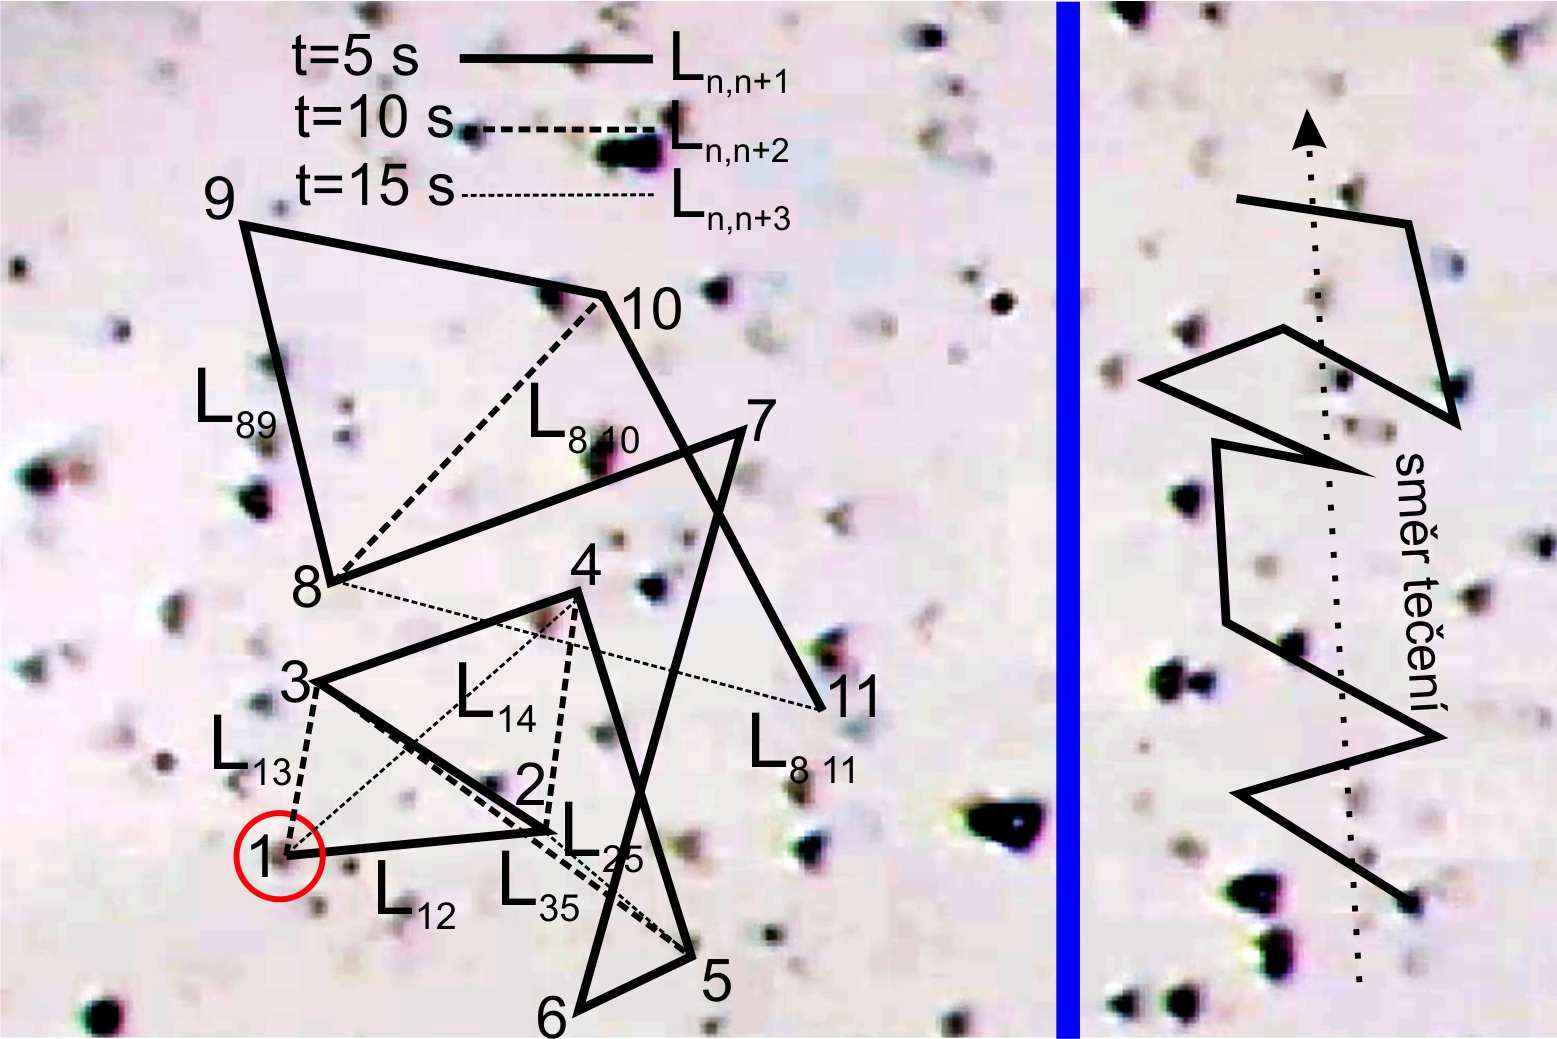
\includegraphics[scale=0.9]{Příklad záznamu chaotického pohybu brownovské částice}
        \captionsetup{justification=centering, font=footnotesize}
        \captionof{figure}{Příklad záznamu chaotického pohybu brownovské částice na průsvitném papíře přiloženém přes obraz z mikroskopu, v případě bez tečení preparátu (vlevo) a při tečení (vpravo). V záznamu pohybu částice vlevo jsou zaneseny trajektorie částice složené z vektorů posunutí při záznamu po časových intervalech t = 5 $s$ (plná čára), 10 $s$ (přerušovaná čára) a 15 $s$ (tečkovaná čára).}
        \label{fig:Příklad záznamu chaotického pohybu brownovské částice na průsvitném papíře přiloženém přes obraz z mikroskopu, v případě bez tečení preparátu (vlevo) a při tečení (vpravo). V záznamu pohybu částice vlevo jsou zaneseny trajektorie částice složené z vektorů posunutí při záznamu po časových intervalech t = 5 s (plná čára), 10 s (přerušovaná čára) a 15 s (tečkovaná čára).}
        \vspace{10pt}
        \raggedright
        \subsection{Pohyblivost volných elektronů v kovu}
            Vodivost kovů spočívá v pohybu nezabraných nositelů náboje, což jsou převážně volné elektrony v kovových materiálech. Hustotu elektrického proudu j můžeme vyjádřit následujícím způsobem:
        \begin{equation}
            j = ne_0 \upsilon_d
        \end{equation}
        kde $\upsilon_d$ je driftová rychlost elektronů, $e_0$ je elementární náboj a $n$ je koncentrace volných elektronů, které se podílení na proudu.
        \par Vzorec pohyblivosti elektronů je následující: 
        \begin{equation}
            \mu = \frac{\upsilon_d}{E}
        \end{equation}
        kde $E$ je intenzita elektrického pole. 
        \par Dosadíme rovnici (20) do rovnice (19):
        \begin{equation}
            j = ne_0 \upsilon_d E = \sigma E = \frac{E}{\rho}
        \end{equation}
        kde $\sigma$ je měrná vodivost a $\rho$ je měrný odpor kovu.
        \par Pak: 
        \begin{equation}
            \sigma = n e_o \mu
        \end{equation}
        Rozhodnout o vztahu mezi teplotou a elektronovou závislostí lze tím, že stanovíme specifickou elektrickou vodivost kovu nebo specifický elektrický odpor pro danou teplotu. Teplotní závislost specifického elektrického odporu $\rho$ se pro malé odchylky teploty $\Delta T$ (na úrovni desítek °C) vůči referenční teplotě přibližuje lineárním vztahem:
        \begin{equation}
            \rho = \rho_0 \left(1 + \alpha \Delta T\right)
        \end{equation}
    \end{minipage}
    \newpage
    \begin{minipage}[t]{0.5\textwidth} 
        kde $\rho_0$ je měrný odpor při refenční teplotě a $\alpha$ je teplotní součinitel odporu. 
        \par Pro drát s odporem $R$, jehož délka je $L$ a plošný průřez má rozlohu $S$, platí následující rovnice:
        \begin{equation}
            R = \frac{L}{\sigma S}
        \end{equation}
        Pak: 
        \begin{equation}
            \mu = \frac{L}{e_0 n R S}
        \end{equation}
        Určení pohybu elektronů lze také popsat pomocí relaxační doby $\tau$. Tuto veličinu můžeme chápat jako průměrnou dobu mezi srážkami elektronu s nečistotami v kovu nebo s rozptylovými procesy na jádrech atomu kovu, které jsou nedejme se tomu, vzhledem k tepelným vibracím atomů, značně rozptýleny. 
        \par Během doby $\tau$ mezi rozptylovými událostmi se elektronův pohyb zrychlí pod vlivem elektrického pole o velikosti $E_0$, což způsobí změnu rychlosti:
        \begin{equation}
            \Delta \upsilon = \frac{e_0 E \tau}{m}
        \end{equation}
        kde $m$ je hmotnost elektronu. 
        \par Po srážce se elektron pohybuje náhodně s náhodným směrem. Právě díky této náhodnosti rozptylových procesů se průměrná rychlost, kterou elektron dosahuje, stává průměrnou rychlostí způsobenou urychlením elektrickým polem. Této rychlosti se říká driftová rychlost:
        \begin{equation}
            \upsilon_d = \frac{e_0 \tau}{m} = \mu E
        \end{equation}
        Pak platí:
        \begin{equation}
            \mu = \frac{e_0 \tau}{m}
        \end{equation}
        \par Dosazením rovnice (28) do rovnice (22) získáme: 
        \begin{equation}
            \sigma = \frac{n e_0^2 \tau}{m}
        \end{equation}
        Koncentrace elektronů je tedy rovna: 
        \begin{equation}
            n = z \frac{\rho}{Am_u}
        \end{equation}
        kde $A$ je atomové hmotnostní číslo prvku a $m_u$ = 1.66 $\times$ $10^{-27}$ kg je atomová hmotnostní jednotka.
        \par Koncentrace některých kovů jsou uvedeny v tabulce (\ref{fig:Hustoty, hmotnostní čísla, počet volných elektronů na jeden atom a koncentrace volných elektronů vybraných kovů}):
        \par
        \vspace{10pt}
        \centering
        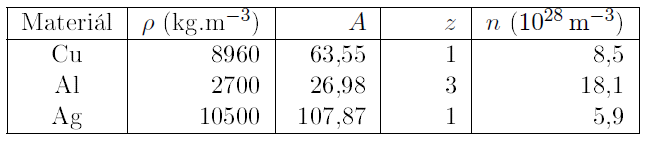
\includegraphics[scale=0.5]{Hustoty, hmotnostní čísla, počet volných elektronů na jeden atom a koncentrace volných elektronů vybraných kovů}
        \captionsetup{justification=centering, font=footnotesize}
        \captionof{figure}{Hustoty, hmotnostní čísla, počet volných elektronů na jeden atom a koncentrace volných elektronů vybraných kovů}
        \label{fig:Hustoty, hmotnostní čísla, počet volných elektronů na jeden atom a koncentrace volných elektronů vybraných kovů}
        \vspace{10pt}
    \end{minipage}
    \hspace{10pt}  
    \begin{minipage}[t]{0.5\textwidth} 
    \section{Měření}  
        \subsection{Brownův pohyb}
        S pomocí skleněné tyčinky vezmeme malé množství temperové běloby. Tuto drobnou porci následně rozpustíme ve vodě, a pomocí téže skleněné tyčinky odebíráme jednu drobnou kapičku roztoku. Tu přeneseme na sklíčko a nakapeme ji uprostřed označené plochy. Poté pokryjeme sklíčkem tak, aby se tekutiny nedotýkalo a nebylo ohraničeno. Takto připravený vzorek vložíme do mikroskopu. 
        \par Začneme pozorovat při malém zvětšení a postupně budeme zvětšovat a zaostřovat. Na obrazovce budeme hledat co největší koncentraci náhodně pohybujících se částic. Poté přiložíme průhlednou fólii k televizní obrazovce a zaznamenáme změny pozice pěti částic s pětivteřinovými intervaly, které budeme měřit pomocí elektrického metronomu. Po zaznamenání pozic vyjmeme vzorek z mikroskopu a umístíme ho do Bürkerovy komůrky. 
        \par Zopakujeme postup jako v předchozí části a na stejném zvětšení, které jsme použili při pozorování částic, najdeme nejmenší čtvereček, u něhož známe přesnou velikost. To nám umožní vypočítat zvětšení mikroskopu. Díky tomu zjistíme velikost jednotlivých tras částic.
        \par Zvětšení mikroskopu se určuje pomocí speciální destičky, která se pod mikroskopem prohlíží. 
        \par Buňku destičky o délce 50 $\mu m$ mikroskop zvětší na délku 12.70(5) $cm$. Určíme zvětšení: 
        \begin{equation}
            x = \frac{12.70(5) cm}{50 \mu m} = 2540(10)
        \end{equation}
        Pro pět částic byly získány následující hodnoty $L_5^2$, $L_{10}^2$ a $L_{15}^2$: 
        \vspace{15pt}
        \par \centering
        \begin{tabular}{|c|c|c|}
            \hline
            $L_5^2$ [$mm^2$] & $L_{10}^2$ [$mm^2$] & $L_{15}^2$ [$mm^2$] \\
            \hline
            121(1) & 400(2) & 784(3) \\
            169(1) & 841(3) & 1600(4) \\
            400(2) & 900(3) & 900(3) \\
            169(1) & 169(1) & 196(1) \\
            81(1) & 16.0(4) & 9.0(3) \\
            121(1) & 100(1) & 100(1) \\
            9.0(3) & 121(1) & 144(1) \\
            121(1) & 324(2) &  \\
            25(1) &  &  \\
            \hline
            \end{tabular}
            \captionsetup{justification=centering, font=footnotesize}
            \captionof{table}{Střední kvadratický posun pro první částici} 
        \vspace{15pt}
        \raggedright
        Odtud zjistíme hodnoty $\left\langle L_{5}^2\right\rangle$, $\left\langle L_{10}^2\right\rangle$ a $\left\langle L_{15}^2\right\rangle$ pro první částici: 
        \begin{center}
            $\left\langle L_{5}^2\right\rangle_1$ = (135 $\pm$ 110)  [$mm^2$]
            \vspace{5pt}
            \par $\left\langle L_{10}^2\right\rangle_1$ = (359 $\pm$ 320)  [$mm^2$]
            \vspace{5pt}
            \par $\left\langle L_{15}^2\right\rangle_1$ = (533 $\pm$ 540)  [$mm^2$]
        \end{center}
    \end{minipage}
\newpage
    \begin{minipage}{0.5\textwidth} 
        \centering
        \begin{tabular}{|c|c|c|}
            \hline
            $L_5^2$ [$mm^2$] & $L_{10}^2$ [$mm^2$] & $L_{15}^2$ [$mm^2$] \\
            \hline
            64(1) & 169(1) & 169(1) \\
            361(2) & 196(1) & 225(2) \\
            100(1) & 529(2) & 256(2) \\
            169(1) & 25(1) & 144(1) \\
            49(1) & 16.0(4) & 100(1) \\
            49(1) & 36(1) & 529(2) \\
            49(1) & 900(3) & 1444(4) \\
            784(3) & 1089(3) &  \\
            169(1) &  &  \\
            \hline
            \end{tabular}
            \captionsetup{justification=centering, font=footnotesize}
            \captionof{table}{Střední kvadratický posun pro druhou částici} 
        \vspace{15pt}
        \raggedright
        Odtud zjistíme hodnoty $\left\langle L_{5}^2\right\rangle$, $\left\langle L_{10}^2\right\rangle$ a $\left\langle L_{15}^2\right\rangle$ pro druhou částici: 
        \begin{center}
            $\left\langle L_{5}^2\right\rangle_2$ = (202 $\pm$ 330) [$mm^2$]
            \vspace{5pt}
            \par $\left\langle L_{10}^2\right\rangle_2$ = (370 $\pm$ 400) [$mm^2$]
            \vspace{5pt}
            \par $\left\langle L_{15}^2\right\rangle_2$ = (410 $\pm$ 440) [$mm^2$]
        \end{center}
        \vspace{15pt}
        \centering
        \begin{tabular}{|c|c|c|}
            \hline
            $L_5^2$ [$mm^2$] & $L_{10}^2$ [$mm^2$] & $L_{15}^2$ [$mm^2$] \\
            \hline
            36(1) & 64(1) & 576(2) \\
            25(1) & 324(2) & 576(2) \\
            256(2) & 529(2) & 529(2) \\
            121(1) & 100(1) & 324(2) \\
            9.0(3) & 144(1) & 144(1) \\
            225(2) & 225(2) & 169(1) \\
            36(1) & 225(2) & 529(2) \\
            81(1) & 400(2) &  \\
            225(2) &  &  \\
            \hline
            \end{tabular}
            \captionsetup{justification=centering, font=footnotesize}
            \captionof{table}{Střední kvadratický posun pro třetí částici} 
        \vspace{15pt}
        \raggedright
        Odtud zjistíme hodnoty $\left\langle L_{5}^2\right\rangle$, $\left\langle L_{10}^2\right\rangle$ a $\left\langle L_{15}^2\right\rangle$ pro třetí částici: 
        \begin{center}
            $\left\langle L_{5}^2\right\rangle_3$ = (113 $\pm$ 90) [$mm^2$]
            \vspace{5pt}
            \par $\left\langle L_{10}^2\right\rangle_3$ = (251 $\pm$ 150) [$mm^2$]
            \vspace{5pt}
            \par $\left\langle L_{15}^2\right\rangle_3$ = (407 $\pm$ 180) [$mm^2$]
        \end{center}
        \vspace{15pt}
        \centering
        \begin{tabular}{|c|c|c|}
            \hline
            $L_5^2$ [$mm^2$] & $L_{10}^2$ [$mm^2$] & $L_{15}^2$ [$mm^2$] \\
            \hline
            36(1) & 100(1) & 25(1) \\
            81(1) & 100(1) & 289(2) \\
            169(1) & 484(2) & 441(2) \\
            81(1) & 121(1) & 400(2) \\
            100(1) & 256(2) & 1225(4) \\
            64(1) & 676(3) & 1024(3) \\
            361(2) & 676(3) & 900(3) \\
            49(1) & 144(1) &  \\
            49(1) &  &  \\
            \hline
            \end{tabular}
            \captionsetup{justification=centering, font=footnotesize}
            \captionof{table}{Střední kvadratický posun pro čtvrtou částici} 
    \end{minipage}
    \hspace{10pt}
    \begin{minipage}{0.5\textwidth} 
        Odtud zjistíme hodnoty $\left\langle L_{5}^2\right\rangle$, $\left\langle L_{10}^2\right\rangle$ a $\left\langle L_{15}^2\right\rangle$ pro čtvrtou částici: 
        \begin{center}
            $\left\langle L_{5}^2\right\rangle_4$ = (110 $\pm$ 100) [$mm^2$]
            \vspace{5pt}
            \par $\left\langle L_{10}^2\right\rangle_4$ = (320 $\pm$ 240) [$mm^2$]
            \vspace{5pt}
            \par $\left\langle L_{15}^2\right\rangle_4$ = (615 $\pm$ 410) [$mm^2$]
        \end{center}
        \vspace{15pt}
        \centering
        \begin{tabular}{|c|c|c|}
            \hline
            $L_5^2$ [$mm^2$] & $L_{10}^2$ [$mm^2$] & $L_{15}^2$ [$mm^2$] \\
            \hline
            256(2) & 144(1) & 49(1) \\
            100(1) & 100(1) & 324(2) \\
            36(1) & 324(2) & 441(2) \\
            144(1) & 256(2) & 121(1) \\
            81(1) & 64(1) & 196(1) \\
            36(1) & 64(1) & 361(2) \\
            25(1) & 324(2) & 676(3) \\
            169(1) & 529(3) &  \\
            100(1) &  &  \\
            \hline
            \end{tabular}
            \captionsetup{justification=centering, font=footnotesize}
            \captionof{table}{Střední kvadratický posun pro pátou částici} 
        \vspace{15pt}
        \raggedright
        Odtud zjistíme hodnoty $\left\langle L_{5}^2\right\rangle$, $\left\langle L_{10}^2\right\rangle$ a $\left\langle L_{15}^2\right\rangle$ pro pátou částici: 
        \begin{center}
            $\left\langle L_{5}^2\right\rangle_5$ = (105 $\pm$ 70) [$mm^2$]
            \vspace{5pt}
            \par $\left\langle L_{10}^2\right\rangle_5$ = (226 $\pm$ 150) [$mm^2$]
            \vspace{5pt}
            \par $\left\langle L_{15}^2\right\rangle_5$ = (310 $\pm$ 200) [$mm^2$]
        \end{center}
        Určeme poměry středních kvadratických posunů pro pět částic: 
        \begin{center}
            $\left\langle L_{5}^2\right\rangle_1$ : $\left\langle L_{10}^2\right\rangle_1$ : $\left\langle L_{15}^2\right\rangle_1$ = 1 : 2.7 : 3.9
            \vspace{5pt}
            \par $\left\langle L_{5}^2\right\rangle_2$ : $\left\langle L_{10}^2\right\rangle_2$ : $\left\langle L_{15}^2\right\rangle_2$ = 1 : 1.8 : 2.0
            \vspace{5pt}
            \par $\left\langle L_{5}^2\right\rangle_3$ : $\left\langle L_{10}^2\right\rangle_3$ : $\left\langle L_{15}^2\right\rangle_3$ = 1 : 2.2 : 3.6
            \vspace{5pt}
            \par $\left\langle L_{5}^2\right\rangle_4$ : $\left\langle L_{10}^2\right\rangle_4$ : $\left\langle L_{15}^2\right\rangle_4$ = 1 : 2.9 : 5.6
            \vspace{5pt}
            \par $\left\langle L_{5}^2\right\rangle_5$ : $\left\langle L_{10}^2\right\rangle_5$ : $\left\langle L_{15}^2\right\rangle_5$ = 1 : 2.1 : 2.9
        \end{center}
        Dále zjistíme poloměr částice $r$ podle vzorce (15). Za $\left\langle x^2 \right\rangle$ dosadíme hodnotu $\left\langle L^2\right\rangle = 2\left\langle x^2 \right\rangle$. Dostaneme: 
        \begin{equation}
            r = \frac{2RT}{3 \left\langle L^2\right\rangle \pi \eta N_A} t
        \end{equation}
        Z tabulkových údajů: 
        \begin{center}
            $R$ = $8.314 \left[\frac{J}{K mol}\right]$
            \vspace{5pt}
            \par $\eta$ = $0.891 \times 10^{-3}$ $\left[\frac{kg}{m s}\right]$
            \vspace{5pt}
            \par $N_A$ = $6.022 \times 10^{23}$ $\left[mol^{-1}\right]$
        \end{center}
        Teplota kapaliny $T$ se rovná pokojové teplotě: 
        \begin{center}
            $T$ = 24.5 [$^\circ$C] = 297.65 [$K$]
        \end{center}
    \end{minipage}
\newpage
    \begin{minipage}[t]{0.5\textwidth} 
    Pak se poloměry těchto pěti částic budou rovnat: 
    \begin{center}
        \centering
        \begin{tabular}{|c|c|c|c|c|}
            \hline
            $r_1$ [$\mu m$] & $r_2$ [$\mu m$] & $r_3$ [$\mu m$] & $r_4$ [$\mu m$] & $r_5$ [$\mu m$] \\
            \hline
            7(6) & 5(5) & 9(7) & 9(8) & 9(6) \\
            3(2) & 3(3) & 4(2) & 3(2) & 4(3) \\
            2(2) & 2(3) & 2(1) & 2(1) & 3(2) \\
            \hline
            \end{tabular}
            \captionsetup{justification=centering, font=footnotesize}
            \captionof{table}{Poloměry pěti částic jsou vypočteny pro hodnoty $\left\langle L_{5}^2\right\rangle$, $\left\langle L_{10}^2\right\rangle$ a $\left\langle L_{15}^2\right\rangle$} 
        \vspace{15pt}
        \raggedright
        Získáme tedy hodnotu $r$:
        \begin{center}
            $r$ = 5(3) [$\mu m$]
        \end{center}
    \end{center}
    \subsection{Pohyblivost volných elektronů v kovu}
        Pro výpočet měrného odporu, měrného odporu $\rho$, měrné vodivosti $\sigma$, pohyblivosti nositelů $\mu$, teplotního součinitela $\alpha$ a střední doby srážek elektronů $\tau$ použijeme vzorce (22), (25), (26), (24) a (28).
        \par Z údajů o zadání: 
        \begin{center}
            $L$ = 29 [$m$]
            \par $R$ = 0.112 [$mm$]
        \end{center}
         Z tabulkových údajů: 
        \begin{center}
            $n_{Cu}$ = $8.5 \times 10^{28} [m^{-3}]$
            \par $e_0$ = $1.6 \times 10^{-19} [C]$
            \par $m_e$ = $9.1093837 \times 10^{-31} [kg]$
        \end{center}
        Výsledky výpočtů jsou uvedeny v tabulce (7).
        \vspace{20pt}
        \par Teplotního součinitel je pak roven:
        \begin{center}
            $\alpha$ = $(3.732 \pm 0.682) \times 10^{-3} [K^{-1}]$
        \end{center}
        Graf závislosti doby srážky elektronů na teplotě: 
        \vspace{20pt}
        \par \centering
        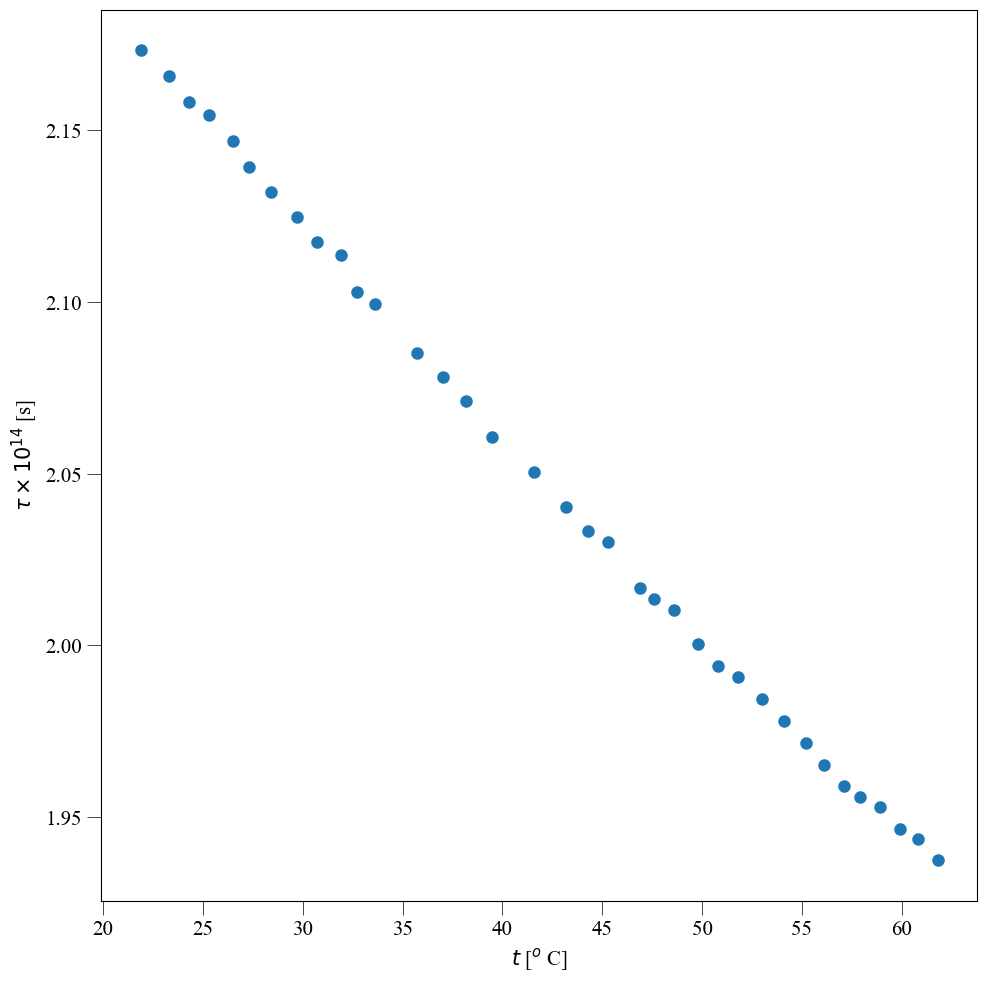
\includegraphics[scale=0.3]{tau}
        \captionsetup{justification=centering, font=footnotesize}
        \captionof{figure}{Graf závislosti doby srážky elektronů na teplotě:}
        \label{fig:Graf závislosti doby srážky elektronů na teplotě:}
        \vspace{10pt}
        \raggedright
    \end{minipage}
    \hspace{10pt}
    \begin{minipage}[t]{0.5\textwidth} 
        K výpočtu nejistot byla použita knihovna "uncertainties" pro Python. 
        \section{Závěr}
            \subsection{Brownův pohyb}
                Získané hodnoty poměrů středních kvadratických posunů částic nesplňují Einsteinův zákon pro první čtyři částice. Pouze pátá částice má poměr $\left\langle L_{5}^2\right\rangle_5$ : $\left\langle L_{10}^2\right\rangle_5$ : $\left\langle L_{15}^2\right\rangle_5$ = 1 : 2.1 : 2.9 odpovídající Einsteinovu zákonu. 
                \par Pravděpodobně je to způsobeno nepřesností definice poloh částic. Například časové intervaly $t$ = 5 [$s$] byly měřeny nesprávně. Také některé polohy částic mohly být nesprávně vyznačeny na samotné obrazovce. 
                \par Poloměr částic $r$ = 5(3) [$\mu m$] je spíše přibližný. 
            \subsection{Pohyblivost volných elektronů v kovu}
                Teplotní součinitel $\alpha$ = $(3.732 \pm 0.682) \times 10^{-3} [K^{-1}]$ poměrně dobře konverguje se svou tabulkovou hodnotou $\alpha$ = $3.92 [K^{-1}]$. Nepřesnost může být způsobena chybou měření odporu při vysokých teplotách.
    \end{minipage}
    \begin{table}[b]
        \centering
        \begin{tabular}{|c|c|c|c|c|c|c|c|}
            \hline
            $T$ $\left[K\right]$ & $\Delta T$ $\left[K\right]$ & $R$ $\left[\Omega \right]$ & $\rho$ $\left[\Omega m \right]$ & $\sigma$ $\left[\Omega^{-1} m^{-1} \right]$ & $\mu$ $\left[\frac{m^2 V}{s} \right]$ & $\alpha$ $[K^{-1}]$ & $\tau$ $[s]$\\
            \hline
            295.05 & -2.6 & 56.7 & 1.926243e-08 & 5.191454e+07 & 0.003817 & -0.000000 & 2.173297e-14\\
            296.45 & -1.2 & 56.9   & 1.933037e-08 & 5.173206e+07 & 0.003804 & -0.002939 &2.165658e-14  \\
            297.45 & -0.2 & 57.1   & 1.939832e-08 & 5.155087e+07 & 0.003791 & -0.035273 &2.158073e-14\\
            298.45 & 0.8 & 57.2  & 1.943229e-08 & 5.146074e+07 &  0.003784 & 0.011023 & 2.154300e-14  \\
            299.65 & 2.0 & 57.4   & 1.950023e-08 & 5.128144e+07  & 0.003771 & 0.006173   &2.146794e-14\\
            300.45 & 2.8 & 57.6   & 1.956818e-08 & 5.110338e+07 & 0.003758 & 0.005669   & 2.139339e-14\\
            301.55 & 3.9 & 57.8   & 1.963612e-08 & 5.092655e+07 &  0.003745 & 0.004974    &  2.131937e-14\\
            302.85 & 5.2 & 58.0   & 1.970407e-08 & 5.075094e+07 & 0.003732 & 0.004409 & 2.124585e-14\\
            303.85 & 6.2   & 58.2   & 1.977201e-08 & 5.057654e+07  &  0.003719 & 0.004267   &2.117284e-14\\
            305.05 & 7.4   & 58.3   & 1.980599e-08 &  5.048978e+07  & 0.003712 & 0.003813 & 2.113653e-14\\
            305.85 & 8.2   & 58.6   & 1.990790e-08 & 5.023130e+07 & 0.003693 & 0.004087   & 2.102832e-14\\
            306.75 & 9.1   & 58.7   & 1.994188e-08 & 5.014573e+07 & 0.003687  & 0.003876  &  2.099250e-14 \\
            308.85 & 11.2   & 59.1   & 2.007777e-08 & 4.980634e+07 & 0.003662 & 0.003779 &   2.085041e-14  \\
            310.15 & 12.5   & 59.3   & 2.014571e-08 & 4.963835e+07 & 0.003650 & 0.003668 &  2.078009e-14  \\
            311.35 & 13.7   & 59.5   & 2.021366e-08 & 4.947150e+07 & 0.003638  & 0.003605   &  2.071024e-14 \\
            312.65 & 15.0   & 59.8   & 2.031557e-08 & 4.922332e+07 & 0.003619  & 0.003645   & 2.060635e-14  \\
            314.75 & 17.1   & 60.1   & 2.041749e-08 & 4.897761e+07 &  0.003601 &0.003507    &  2.050349e-14  \\
            316.35 & 18.7   & 60.4   & 2.051941e-08 & 4.873434e+07 & 0.003583 & 0.003490   &  2.040165e-14 \\
            317.45 & 19.8   & 60.6   & 2.058735e-08 & 4.857351e+07 & 0.003572  & 0.003474   &  2.033432e-14 \\
            318.45 & 20.8   & 60.7   & 2.062133e-08  & 4.857351e+07 & 0.003566  & 0.003392   &  2.030082e-14  \\
            320.05 & 22.4   & 61.1   & 2.075722e-08 & 4.817601e+07 &  0.003542 & 0.003464   &  2.016791e-14 \\
            320.75 & 23.1   & 61.2   & 2.079119e-08 & 4.809729e+07 & 0.003537 & 0.003436   &  2.013496e-14  \\
            321.75 & 24.1   & 61.3   & 2.082516e-08 & 4.801883e+07 & 0.003531  & 0.003366   &  2.010211e-14  \\
            322.95 & 25.3   & 61.6 & 2.092708e-08  & 4.778497e+07 &  0.003514 & 0.003416   &  2.000421e-14  \\
            323.95 & 26.3   & 61.8   & 2.099503e-08 & 4.763033e+07 & 0.003502  & 0.003420   &  1.993947e-14 \\
            324.95 & 27.3 & 61.9   & 2.102900e-08 & 4.755338e+07 &  0.003497 & 0.003359   & 1.990726e-14   \\
            326.15 & 28.5   & 62.1   & 2.109694e-08 & 4.740023e+07 &  0.003485  & 0.003342   & 1.984315e-14 \\
            327.25 & 29.6   & 62.3   & 2.116489e-08 & 4.724806e+07 &  0.003474  & 0.003337   & 1.977945e-14  \\
            328.35 & 30.7   & 62.5   & 2.123283e-08  & 4.709687e+07 &  0.003463  & 0.003332   & 1.971615e-14 \\
            329.25 & 31.6   & 62.7   & 2.130078e-08 &4.694664e+07 & 0.003452 & 0.003349   &  1.965326e-14   \\
            330.25 & 32.6 & 62.9   &  2.136872e-08 & 4.679737e+07 & 0.003441  & 0.003354   & 1.959077e-14   \\
            331.05 & 33.4   & 63.0   & 2.140270e-08 & 4.672309e+07 & 0.003436  &0.003327    &  1.955967e-14 \\
            332.05 & 34.4   & 63.1    & 2.143667e-08 & 4.664904e+07 & 0.003430  & 0.003281   & 1.952868e-14   \\
            333.05 & 35.4 & 63.3   & 2.150461e-08  & 4.650165e+07 & 0.003419  & 0.003288   &  1.946697e-14 \\
            333.95 & 36.3   & 63.4   & 2.153859e-08 & 4.642830e+07  & 0.003414  & 0.003255   & 1.943627e-14 \\
            334.95 & 37.3   & 63.6   & 2.160653e-08  & 4.628230e+07 &  0.003403  & 0.003263   & 1.937515e-14  \\
            \hline
            \end{tabular}
            \captionsetup{justification=centering, font=footnotesize}
            \captionof{table}{Hodnoty teploty $T$, odporu $R$, rozdílu mezi pokojovou teplotou $\Delta T$, měrného odporu $\rho$, měrné vodivosti $\sigma$, pohyblivosti nositelů $\mu$ teplotního součinitela $\alpha$ a střední doby srážek elektronů $\tau$} 
    \end{table}
\end{document}